\section{The Système de Contrôle Distribué}
\label{sec:scd}
Real-time control is a fundamental requirement in modern tokamak operation. The Système de Contrôle Distribué (SCD) \cite{le_distributed_2014,anand_distributed_2017,galperti_overview_2024} represents a distributed real-time control architecture designed for the TCV tokamak. The system emerged from the necessity to handle a considerable number of actuators and diagnostics while maintaining precise control over plasma behavior. Its distributed nature, of particular interest in this work, stems from the need to minimize analog signal paths across the facility, employing real-time-capable networks to interconnect various subsystems.

The SCD interfaces with hundreds of diagnostic channels while controlling multiple actuator systems. These include independently controllable coil power supplies, steerable real-time Electron Cyclotron launchers with continuously variable power, multiple neutral beam injectors, and an array of gas injection valves. Such an extensive set of controllable elements demands a sophisticated control infrastructure capable of coordinating multiple operations simultaneously.

A distinctive characteristic of TCV operation lies in the fast plasma dynamics, which imposes stringent timing requirements on the control system. Despite its relatively small size compared to future reactor designs, TCV requires primary magnetic control loops executing within \SI{100}{\micro\second}. This temporal constraint represents a defining factor in the system architecture, influencing both hardware and software designs.

The SCD design philosophy emphasizes two seemingly contrasting requirements: operational flexibility and system reliability. The control infrastructure should facilitate rapid implementation and testing of novel control schemes while maintaining robust operation during regular experimental campaigns. This duality led to the adoption of MATLAB/Simulink as the primary development environment, enabling control algorithm prototyping through graphical programming and subsequent automated code generation.

The initial implementation of the SCD, now more than a decade old, required a complete  recompilation of the control code before each plasma discharge when control parameters were modified. While this approach supported the exploratory phase of the SCD implementation, it proved increasingly difficult to maintain as the system expanded and the number of integrated modules and algorithms increased.

The transition to the MARTe2 framework (see \Cref{sec:related_work_marte2}) marked a significant improvement, introducing a modular, maintainable architecture with enhanced standardization capabilities. MARTe2, specifically designed for fusion applications, provides a comprehensive environment for real-time software applications. Its data-driven runtime workflow enables dynamic parameter and waveform loading during the initialization of a discharge, eliminating the need for frequent recompilations. This framework has also improved the integration between real-time computers and the TCV IT infrastructure, streamlining the deployment of new control algorithms from development to experimental validation.

The SCD hardware architecture comprises multiple computational nodes interconnected through dedicated networks. The main processing units consist of industrial PCs operating under real-time Linux, specifically customized with the \texttt{PREEMPT\_RT} patch, CPU isolation, and specialized kernel parameters. These modifications enable deterministic operation while maintaining a conventional operating system environment, avoiding the complexity of custom-compiled kernels. A summary schematic of the system is given in \Cref{fig:scd}.

Input and output operations rely on high-density ADC/DAC modules. A dedicated reflective memory network (RFM) provides communication at \SI{170}{\mega\byte/\second} with sub-microsecond latency between computational nodes. This infrastructure is complemented by an EtherCAT real-time industrial network deployed to manage distributed low-count I/O subsystems, each handling up to 10 analog channels, with a total capacity of approximately 500 channels. The computational nodes, each performing specific functions in the control architecture, are organized as follows.
\begin{itemize}
  \item \textbf{Node 01} operates the Far Infra Red interferometer (FIR) and related X ray diagnostics.
  \item \textbf{Node 02} and \textbf{Node 03} constitute the main control nodes of the system. Node 02 serves as the primary controller while Node 03 acts as its twin for debugging and backup purposes, \emph{i.e.}, it runs the same code on the same hardware reading the same measurements but it is not connected to any actuator. These nodes manage all coils, gas valves, and auxiliary heating systems.
  \item \textbf{Nodes 05} and \textbf{Node 06} provide computational capabilities through 6-core  Intel Core~i7 processors. One unit incorporates a real-time network analyzer to monitor the performance of the reflective memory network.
  \item \textbf{Node 07} executes real-time MHD analysis, monitoring rotating tearing modes and locked modes.
  \item \textbf{Node 08} handles fast acquisition and real-time processing of Electron Cyclotron Emission data.
  \item \textbf{Node 09} manages real-time acquisition and processing of the Thomson scattering diagnostic, providing calibrated electron temperature and density profiles.
  \item \textbf{Node 10}, designated as MANTIS, operates a sophisticated 10-camera multispectral imaging system. It captures spectrally filtered tangential images of the plasma at frequencies between \SI{200}{\hertz} and \SI{800}{\hertz}, enabling real-time processing for applications such as radiation front position estimation along the divertor.
\end{itemize}
The primary control functionality, implemented on Node 02 with Node 03 as backup, represents a critical component of the system. This subsystem interfaces with a 192-channel ADC module, sending data streams through two high-speed fiber optic links to both the industrial PCs that implement the nodes. This redundant configuration ensures synchronized data delivery to both nodes, enabling parallel operation during plasma discharges.

A central server orchestrates the entire control system, managing a main shot state machine that coordinates all distributed computers. This server maintains an MDSplus database (see \Cref{sec:related_work_marte2}) containing control system data and real-time algorithm configurations, hosts the development environment for control algorithm implementation and provides a secure platform for authorized users to integrate new controllers into the TCV control framework.

\begin{figure}[t!]
  \centering
  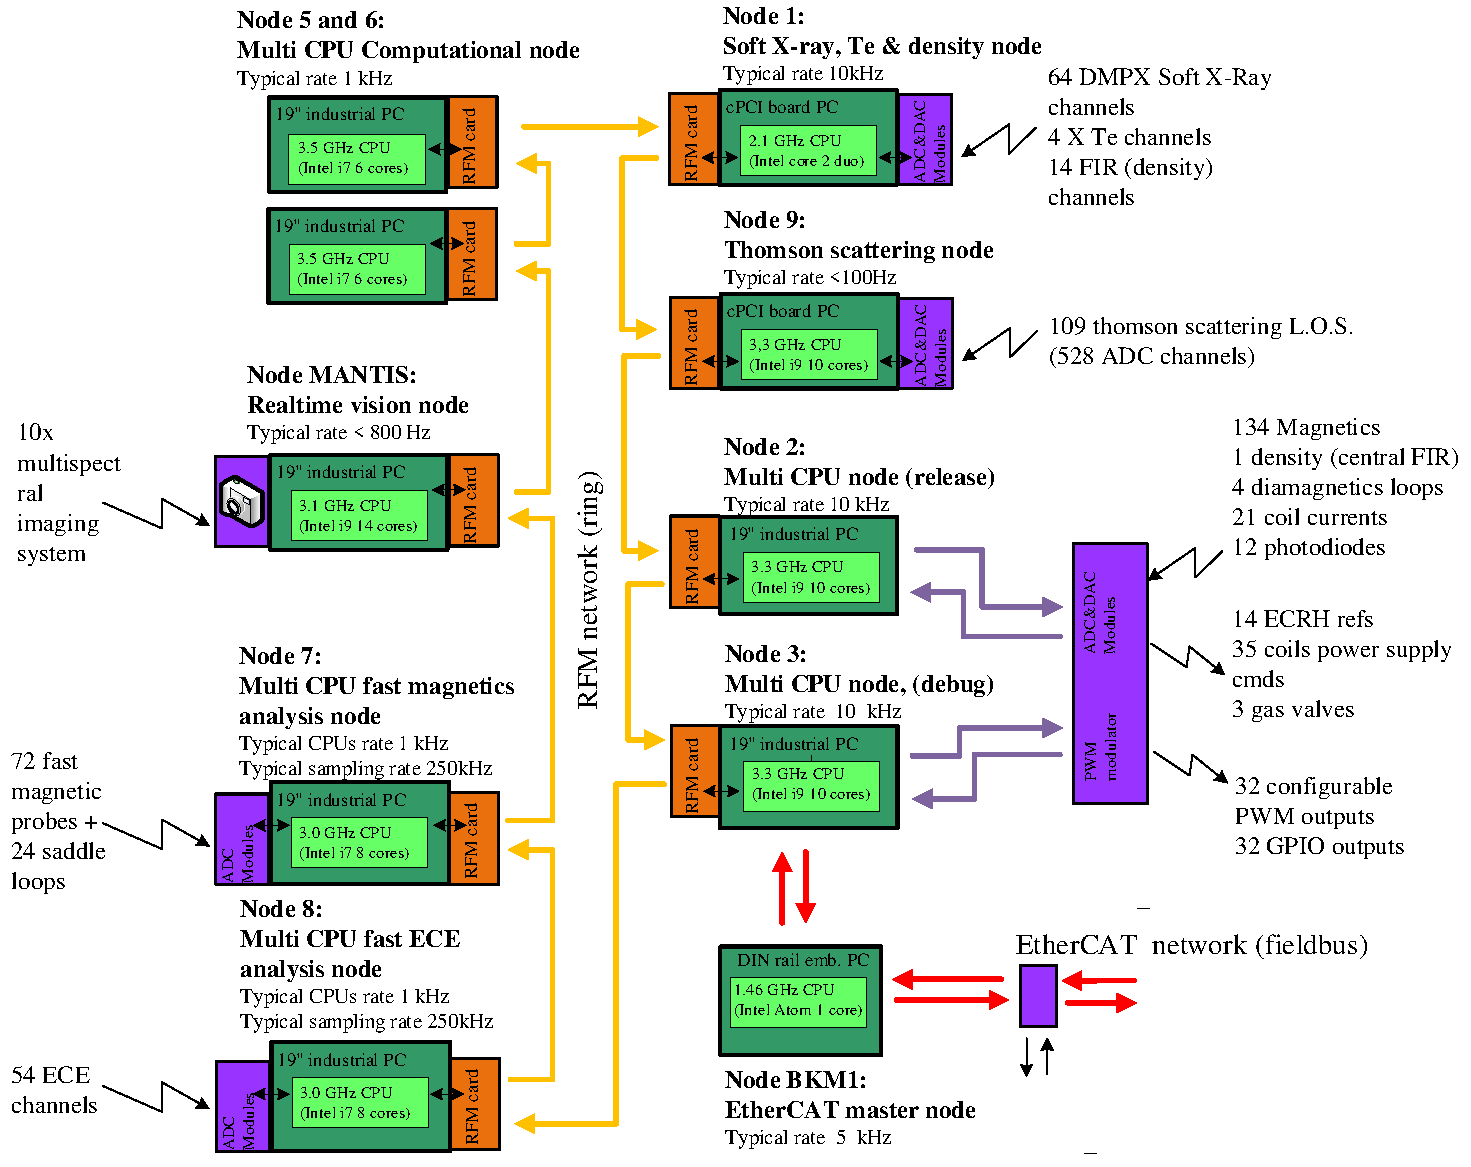
\includegraphics[width=\textwidth]{images/ch6/SCD.pdf}
  \caption{Schematic of the Système de Contrôle Distribué (SCD) architecture.}
  \label{fig:scd}
\end{figure}

The software development workflow employs an object-oriented simulation framework, designated as SCDDS (Simulink-based Control Design and Deployment Suite), which manages parameter and waveform access consistently between simulation and real-time environments. After new algorithms have been developed with the graphical programming tools offered by MATLAB/Simulink, the SCDDS framework handles the complexity of parameter management, enabling developers to focus on control logic implementation. This approach proves particularly valuable when validating new algorithms using historical plasma discharge data. Once validated in simulation, control algorithms undergo automated code generation, producing C code that replicates the behavior of the original Simulink design. The SCDDS framework ensures a streamlined integration process within the MARTe2 environment, in which the entirety of the real-time control algorithms run to ensure that the system satisfies the stringent timing requirements in a deterministic fashion.
